\subsection{Fixation de \(\alpha\)}

\subsubsection{Configuration, modifications et résultats attendus}

Nous savons que pour un \emph{Soft Actor Critic} le paramètre \(\alpha\) gérant
l'entropie peut être fixé ou non en fonction du problème. Jusque maintenant,
nous faisions apprendre ce paramètre à l'algorithme. Nous souhaitons désormais tester les performances avec une valeur de $0.02$. On espère que l'évolution des fonctions de pertes soit plus efficace.

\subsubsection{Analyse}

\begin{figure}[H]
    \centering
    \begin{subfigure}{0.45\textwidth}
        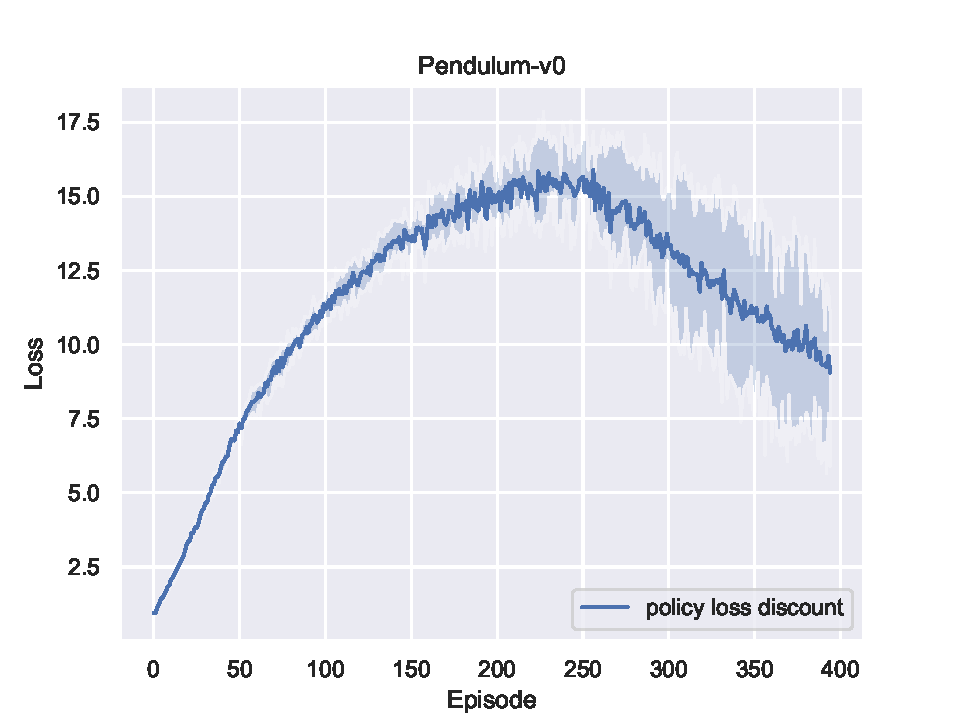
\includegraphics[width=\textwidth]{figures/sac_itr3/policy_loss_Pendulum-v0_pg_dataset_td_trajs_400_update_threshold_1000_nb_updates_20_gamma_0.98_tau_0.01_nstep_5_lr_act_0.0005_lr_critic_0.001_init_alpha_0.02_lr_alpha_0.0_target_entropy_alpha_-1.0pg.pdf}
        \caption{Fonction de perte de la politique}
    \end{subfigure}
    \begin{subfigure}{0.45\textwidth}
        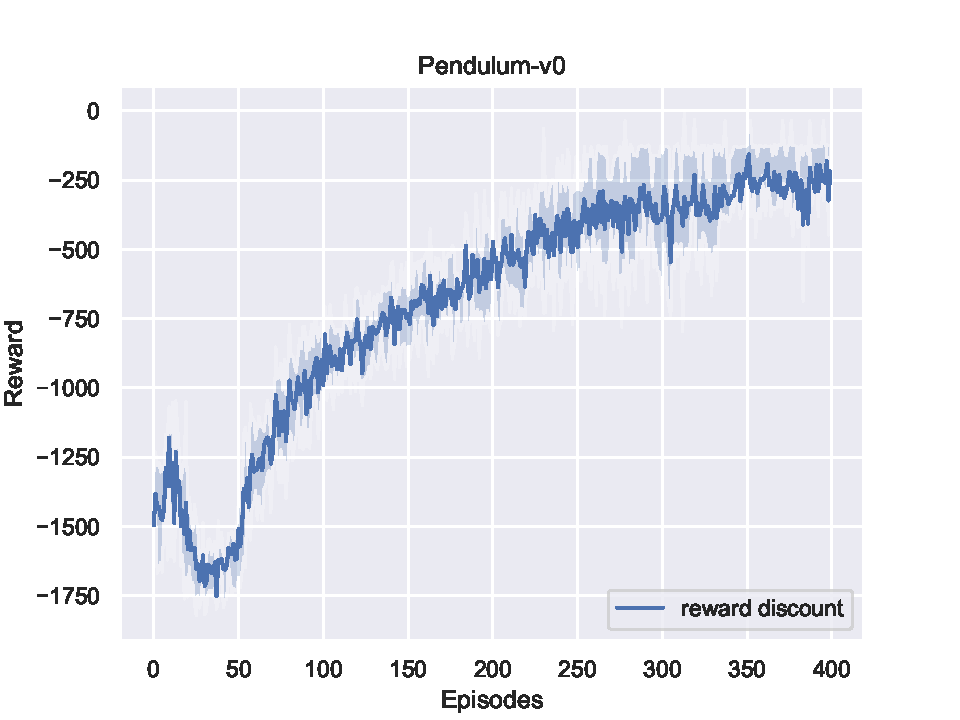
\includegraphics[width=\textwidth]{figures/sac_itr3/rewards_Pendulum-v0_pg_dataset_td_trajs_400_update_threshold_1000_nb_updates_20_gamma_0.98_tau_0.01_nstep_5_lr_act_0.0005_lr_critic_0.001_init_alpha_0.02_lr_alpha_0.0_target_entropy_alpha_-1.0.pdf}
        \caption{Les récompenses de la politique}
    \end{subfigure}
    \caption{Résultats obtenus pour la politique et la récompense}
    \label{fig:sac:results3}
\end{figure}

La récompense de la politique semble arriver plus rapidement à un score de $-250$ avec $\alpha$ fixé que lorsqu'il est appris. De plus, la fonction de perte de la politique décroit également plus rapidement. 

Avec seulement $400$ épisodes, les courbes des fonctions de coût des deux critiques de SAC ne sont pas bien différente de l'étude précédente (fig~\ref{fig:sac:results2}). Les graphes des valeurs de la politique et des critiques sont très ressemblantes à celles déjà obtenues. Nous avons jugé non nécessaire de les présenter ici.